\section{Support Vector Machine}

\subsection{Methods}
\subsubsection{Treatment of Data}
\paragraph{Splitting}
For the implementation of the SMO algorithm the training data had not to be split into fixed training and validation sets. Instead the imperative was to implement 10-fold crossvalidation for parameter selection of $\tau$ and C. In order to achieve this task and save time we used the KFold() method of the python scikit library. This method thus splits the dataset into 10 consecutive folds without shuffling. Each fold is then used once as a validation set while the k-1 remaining folds form the training set.
\paragraph{Preprocessing}
Regarding preprocessing we applied the same normalization as with the Multilayer Perceptron.

\subsubsection{SVM setup}
To determine the optimal parametrization of the SVM we ran the SMO algorithm with 10-fold crossvalidation for the following range of values of $C$ and $\tau$:
\begin{tabular}{l|llllllllll} 
	\toprule
	$\tau$ & 0.002 & 0.004 & 0.008 & 0.016 & 0.032 & 0.064 & 0.128 & 0.256 & 0.512 \\
	C & 1 & 2 & 4 & 8 & 16 & 32 & 64 & 128 & 256 & 512 \\
	\bottomrule
\end{tabular}

\subsection{Results}
Resulting scores from the crossvalidation
\begin{figure}[!ht]
	\centering
	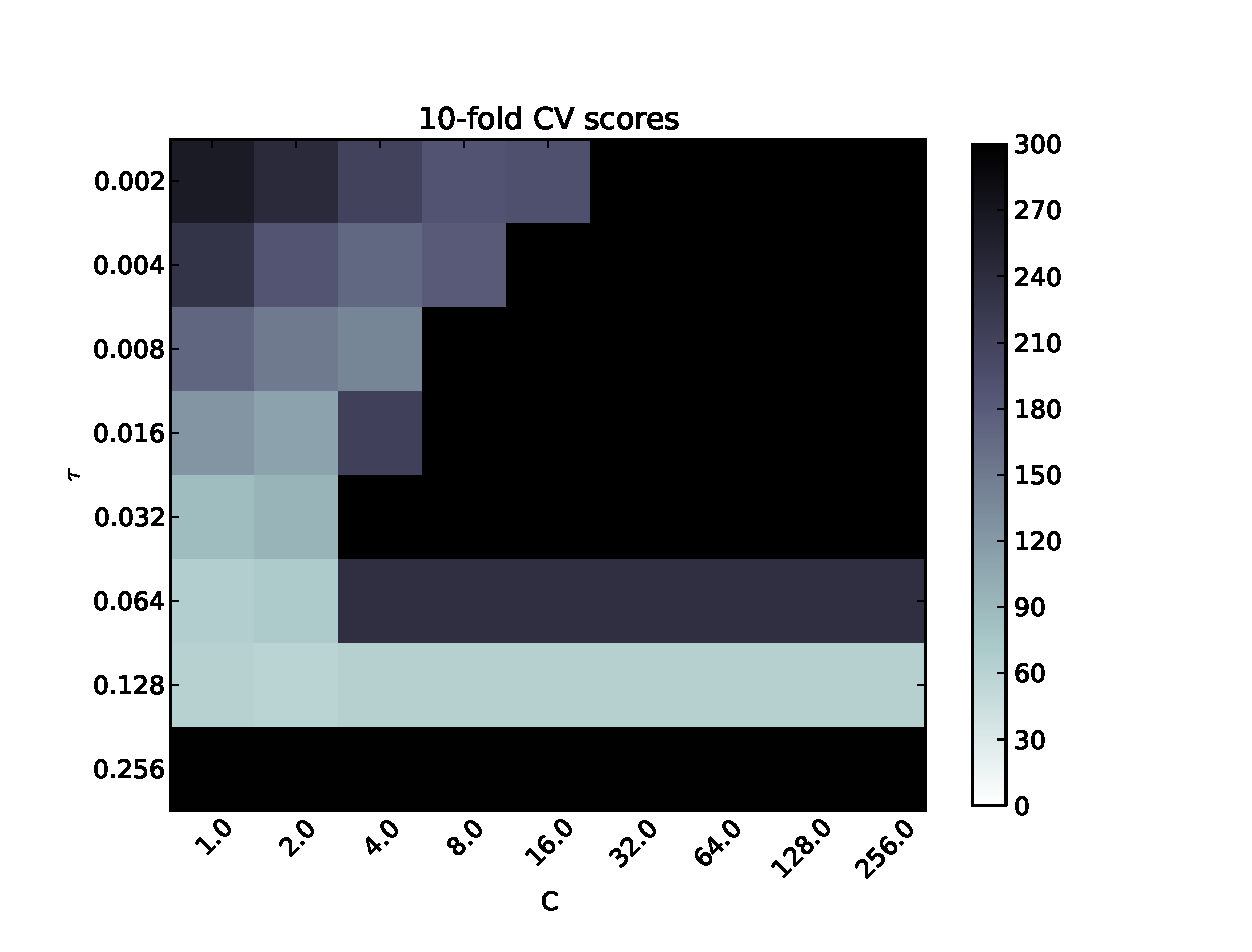
\includegraphics[width=.6\textwidth]{svm/scores_max_300.eps}
	\label{fig:scores}
	\caption{Summed up misclassification scores for range of parameters $C$ and $\tau$ depicted after 10-fold crossvalidation. The smallest total score was recorded for $\tau=.128$ and $C=2$. The range of values is displayed up to a maximum score of 300 which represents 5\% misclassifications on the validation data over the 10 folds.}
\end{figure}

\subsection{SVM criterion and Convergence criterion}
Plot the SVM criterion as function of SMddO iterations (only
every 20 SMO steps). Additionally, plot the value of the convergence criterion,
based on KKT condition violations (see additional note). For the latter plot,
the vertical axis should have a logarithmic scale.
\section{Performance comparison of SVM and MLP}
Comparison of the final setup of the Multilayer Perceptron and Support Vector Machine. In fig. .. we displayed the training and testing zero-one errors for the final parametrizations as required. One can see that SVM performs better overall...

\begin{figure}[!ht]
	\centering
	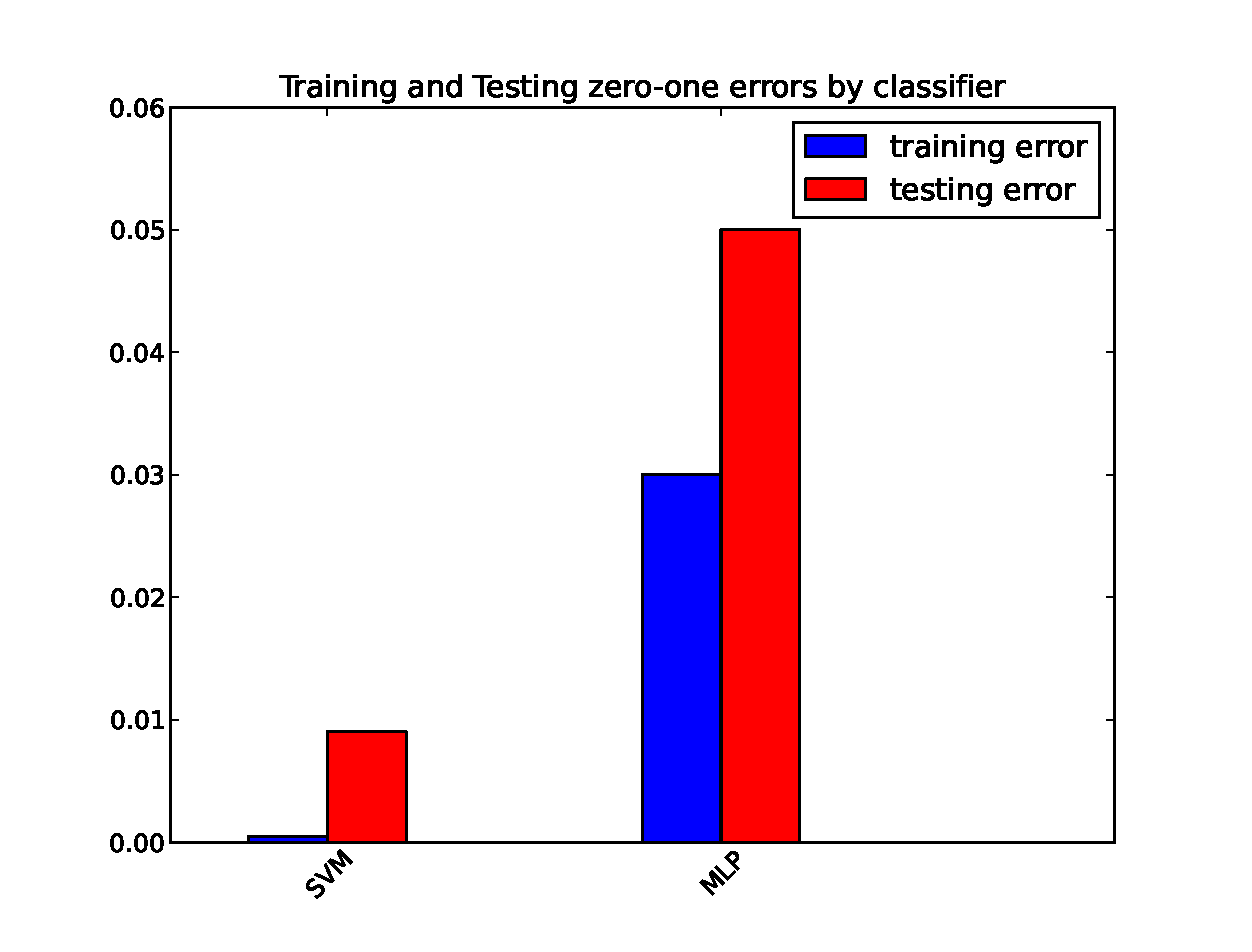
\includegraphics[width=\textwidth]{svm/fake_bar_plot.eps}
	\caption{bar plot of zero-one error for training and testing comparing MLP ( h1=.., eta=, mu=)and SVM (tau=.. and C=.. )}
	\label{fig:comparison}
\end{figure}